\chapter{Theoretical background}
\label{chap:Background}
\mtoc

In this chapter, we provide a brief overview of the main concepts of natural language processing required to understand the rest of this work.

\section{Language models}
\label{sec:Background-LanguageModels}

Language models are probabilistic models that predict the next word in a sequence. They also assign probabilities all possible sentences and sequences of words constructed from the words of a given language (\cite{Jura09}).

We train language models on large corpora of text written in a given language. For example, by counting occurrences and co-occurrences of words. A language model trained on a big enough English corpora should assign a higher probability to the first sentence and consider the second one very unlikely.

\begin{enumerate}
\item Today is a rainy day here in Paris.
\item Nice not such but inside in after.
\end{enumerate}

Finding the probability distribution of words is an important part of many NLP problems, such as spellchecking, error correction, or machine translation. As we will see in Section \ref{sec:Background-seq2seq}, state of the art recurrent neural network used for machine translation are also very advanced language models.

\section{Entropy and cross-entropy}

The amount of information produced when one message is chosen from the set of possible messages can be measured as

\[ I(x) = -log_2 P(x) \]

It was \cite{Shan48} who proposed to use the logarithm with base 2 and call the units of information bits (or binary digits). We can also use natural logarithm but then the units of measurement will be called nats.

\subsection{Entropy}

In information theory, a random variable is treated as a source of information. The entropy of variable X is the expectation of the amount of information in the outcome (\cite{Mack03}).

\[ H(X) = \mathbb{E}\big[ I(x) \big] = - \mathbb{E}\big[ log P(x) \big] \]

In the context of languages, we only consider discrete random variables over the finite alphabet.

\[ H(X) = - \sum_{i=1}^N P(x_i) log P(x_i) \]

Entropy is considered the measure of uncertainty of variable X.

\subsection{Kullback-Leibler divergence}
\label{sec:Background-KL}

The difference between two probability distributions is measured with a Kullback-Leibler (KL) divergence:

\[ D_{KL}(P||Q) = \mathbb{E}\bigg[ \log \frac{P(x_i)}{Q(x_i)} \bigg] = \mathbb{E}\big[ \log P(x_i) - \log Q(x_i) \big] \]

For the case of discrete variables

\[ D_{KL}(P||Q) = \sum_{i=1}^N P(x_i) \log \frac{P(x_i)}{Q(x_i)} \]

\subsection{Cross-entropy}

Cross-entropy is the average number of bits needed to encode data from the source with distribution P when we use model Q to define our codebook (\cite{Murp13}).

\[ H(P, Q) = - \sum_{i=1}^N P(x_i) log Q(x_i) \]

It can be expressed as a sum of entropy and KL divergence

\begin{equation}
    H(P, Q) = H(P) + D_{KL}(P||Q)
    \label{eq:KL-Entropy}
\end{equation}

The lower bound of cross-entropy means that even if we find the perfect model which matches the true distribution of data, cross-entropy will not be lower than the entropy of this dataset.

\subsection{Why do we minimize the cross-entropy?}
\label{sec:Background-Likelihood}

Many problems in machine learning can be viewed as function estimation: we are trying to predict a variable $y$ given an input vector $x$ (\cite{Good16}). We assume that there is a true function $f(x)$ that describes relationship between $x$ and $y$. All other factors that influence $y$ are considered to be noise $\epsilon$ (in real world nothing is really influenced by a single factor; be it a coin toss or a roll of dice, outcome of any process is affected by more factors than we could possibly measure, however, the effect of most factors is so insignificant that they can be ignored).

\[ y = f(x) + \epsilon \]

We want to find function $\hat{f}$ (model, estimate) which is as close as possible to the "true" function $f$. When we say that we are training a machine learning model, we mean that we choose a model, which is a parametrised function $\hat{f}(x;\theta)$ and iteratively move it closer to the "true" function $f$ by changing the parameter $\theta$.

In probabilistic interpretation the process that we are trying to model, or function $f$, is the "true" probability distribution $P_{data}(x, y)$ that generates a set of $(x, y)$ points. We observe this process by collecting the training data $D =\{(x^{(i)}, y^{(i)})|i=1,2,\dots\}$ and try to model it with a parametric family of distribution $P_{model}(x, y; \theta)$ (function $\hat{f}$) by finding such parameter $\theta^{*}$ which minimizes the difference between those two distributions. As we mentioned in Section \ref{sec:Background-KL}, the difference between two distributions is measured with a Kullback-Leibler divergence.

\[ \theta^{*} = \argmin_{\theta} D_{KL}(P_{data}||P_{model}) \]

And based on Equation \ref{eq:KL-Entropy}, this is the same as minimizing the difference between the cross-entropy of our model applied to the dataset $H(P_{data}, P_{model})$ and the entropy of this dataset $H(P_{data})$

\[ \theta^{*} = \argmin_{\theta} \bigg[H(P_{data}, P_{model}) - H(P_{data})\bigg] \]

Since $P_{data}$ does not depend on $\theta$ and can not be controlled by us, this boils down to minimizing the cross-entropy:

\[ \theta^{*} = \argmin_{\theta} H(P_{data}, P_{model}) \]

Now we will show that this is the same as maximizing the likelihood of the dataset $D$ assigned to it by our model $P_{model}$. The likelihood is the measure of how likely is our model to produce this dataset. We assume that by choosing the model which has highest likelihood of generating dataset $D$ we will get a model that behaves like the true process in other situations (this really depends on how representative is $D$ of the entire distribution $P_{model}$ and whether we are able to generalize and not overfit - simply memorize - the training data $D$). The likelihood is expressed as the probability that our model $P_{model}$ assigns to the dataset $D$. So we want to find parameter $\theta^{*}$ which maximizes this probability:

\[ \theta^{*} = \argmax_{\theta} P_{model}(D;\theta) \]

We make an assumption that all points in $D$ are independent of each other, which allows us to express the probability of generating dataset $D$ into the product of probabilities of generating each one of its points. If $m = |D|$ is the size of our dataset,

\[ P_{model}(D;\theta) = \prod_{i=1}^m P_{model}(x^{(i)}, y^{(i)};\theta) \]

Which means that

\[ \theta^{*} = \argmax_{\theta} \prod_{i=1}^m P_{model}(x^{(i)}, y^{(i)};\theta) \]

To simplify this task, we can use the property of logarithms which turns product into a sum, and maximize the logarithm of expression on the right. Indeed the same parameter $\theta^{*}$ which maximizes the logarithm of an expession, will also maximize that expression. Therefore,

 \[ \theta^{*} = \argmax_{\theta} \log \prod_{i=1}^m P_{model}(x^{(i)}, y^{(i)};\theta) \]
 \[ = \sum_{i=1}^m \log P_{model}(x^{(i)}, y^{(i)};\theta) \]

 The logarithm of a likelihood (right-hand side expression) is called log-likelihood. In the same way, we can multiply this expression by any constant without changing the maximization parameter. Let's normalize it over the size of our dataset

 \[ \theta^{*} = \argmax_{\theta} \frac{1}{m}\sum_{i=1}^m \log P_{model}(x^{(i)}, y^{(i)};\theta) \]

 This, in fact is the expectation of log-pobability of random point with respect to the probability distribution $P_{data}$:

 \[ \theta^{*} = \argmax_{\theta} \mathbb{E}_{(x,y) \sim P_{data}} \bigg[\log P_{model}(x, y;\theta)\bigg] \]

 Which is the same as minimizing the negative expectation, or cross-entropy:

 \[ \theta^{*} = \argmin_{\theta} - \mathbb{E}_{(x,y) \sim P_{data}} \bigg[\log P_{model}(x, y;\theta)\bigg] \]

  \[ = \argmin_{\theta} H(P_{data}, P_{model}) \]

This explains why we train machine learning models by minimizing cross-entropy and why it is the same as maximizing the likelihood. Every cost function is, in fact, the cross-entropy of empirical distribution $P_{data}$ and some the distribution that we choose for our model. For example, mean squared error (MSE) is cross-entropy of $P_{data}$ and the normal distribution.

\section{Recurrent neural networks}
\label{sec:Background-RNN}

A big limitation of feedforward neural networks is the fact that they require a fixed-size input and always produce a fixed-size output. For example, a network that has 2 neurons in the input layer and 1 neuron in the output layer can only accept vectors of size 2 and return vectors of size 1.

Some problems, however, require processing of sequential data. This includes time series forecasting, music composition, and many tasks of natural language processing, such as machine translation, text summarization, question answering, sentiment analysis, speech recognition, text-to-speech and speech-to-text translation etc. The input of these problems is a sequence of variable length.

\textbf{Recurrent neural networks} (RNN) are a special kind of neural networks that have cyclical connections. At every step, such networks receive a fixed-size input (for example, one word) and the information from the previous step, transmitted through the cyclical connection. This creates memory inside a network which allows it to operate on sequences of input values.

\begin{figure}[H]
    \label{fig:rnn}
    \centering
    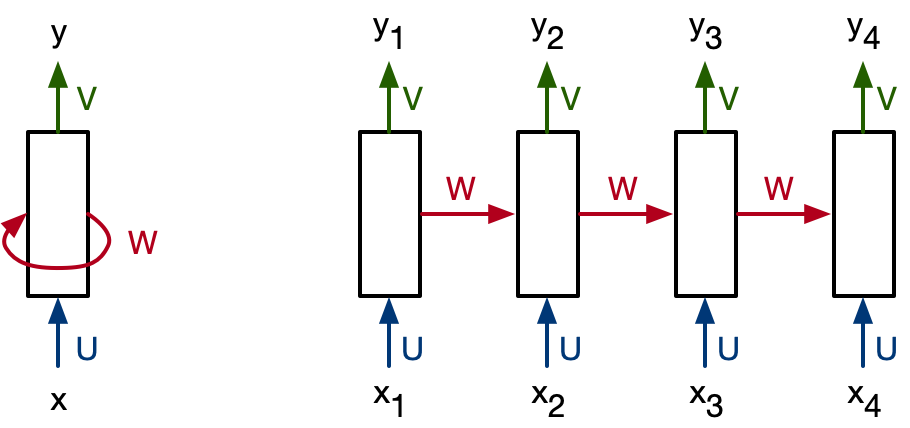
\includegraphics[height=4cm]{rnn}
\end{figure}

\subsection{Sequence to sequence networks}
\label{sec:Background-seq2seq}

On each step, recurrent neural network receives an input value, produces the output value, and passes its internal state onto the next step. From this follows:

\begin{enumerate}
    \item Sequence of $N$ inputs will produce a sequence of $N$ outputs.
    \item Every output $y_k$ is only affected by the current input $x_k$ and all the previous inputs $x_1, \dots x_{k-1}$ but not the next inputs $x_{k+1}, \dots, x_N$
\end{enumerate}

This is useful for problems like predicting next element in a sequence, but other tasks may require input and output sequences to be of different sizes and the output to be equally affected by all elements of input.

Consider a question answering system. A neural network receives a sequence of words in a question: \textit{"At what temperature does water boil?"} and produces the answer: \textit{"Water boils at 100 degrees."}. Such answer cannot be produced by a classical RNN because the length of a question exceeds the length of the answer and it is impossible to produce the beginning of the answer \textit{"Water boils ..."} until we have seen the end of the question \textit{"... does water boil"}.

This can be done by a special combination of two recurrent neural network called \textbf{sequence to sequence} or \textbf{encoder-decoder neural network} neural networks introduced by \cite{Suts14}.

\paragraph{Encoder} is a recurrent neural network which accepts the sequence of input values. The output of encoder is ignored and the state vector received on the last step encodes the input sequence (sometimes called "thought vector").

\paragraph{Decoder} is another recurrent neural network which receives its own output from the previous step as input on the current step and generates the output sequence. On the first step, a decoder receives the encoded sequence provided by the encoder as its internal state.

Putting encoder and decoder together we receive a neural network which first reads the whole input sequence of size $N$ and only then produces the output sequence of size $M$, making it possible that $N \neq M$.

Sequence to sequence networks are in fact language models that learn the probability distribution of the output sequences conditioned by the input sequences. They are widely used in machine translation, question answering, text summarization, and many other similar applications.

\subsection{LSTM and GRU cells}
\label{sec:Background-LSTMandGRU}

The major problem with recurrent neural networks is vanishing or exploding gradient. As the network is trained on a sequence of input, we use the algorithm called "backpropagation through time" which propagates an error back through the cyclical connection reversing the path made by the input sequence. This process is similar to backpropagating an error through the deep feedforward network with as many layers as the length of the input sequence. The only difference is that the weight matrix on each layer is now the same matrix corresponding to the cyclical connection. This leads to the problem described by \cite{Hoch01}: backpropagated error signals exponentially depend on the magnitude of weights. They tend to either explode if weights are above 1 or vanish if they are below.

As a solution to this problem \cite{Hoch97} introduced a novel method called \textbf{Long short-term memory (LSTM)} - memory cells with internal architecture that allows bridging very long time lags and does not suffer from exploding or vanishing gradient.

\cite{Cho14} proposed a simplified version of memory cells called \textbf{Gated recurrent unit (GRU)} which achieve similar performance to LSTM cells but have fewer parameters.
